\section{Introduction}
\label{sec:intro}

This report uses the \emph{how much did it rain ii} \cite{rain, Lakshmanan16}
dataset from \emph{kaggle.com} for the analysis of different sketching methods.
The original dataset contains 13,765,201 training samples
with 23 features and 1 prediction value.
See the Appendix for detailed description of features.
Since it contains null values, and outliers,
we will do a preprocess and only use a subset of samples.

\subsection{Baseline and Preprocess}

Since some observations are not complete,
we first filter out 2,769,088 samples that do not contain missing values.
The first two features \emph{id} and \emph{minutes\_past}
are used just for identification rows,
thus we omit them and
get data matrices
\begin{equation}
    A_0 \in \real^{2769088\times 21}, \,
    b_0\in\real^{2769088}
\end{equation}

Let's look at the distribution of these features first.
Figure~\ref{fig:box}
\begin{figure}[t]
	\centering
	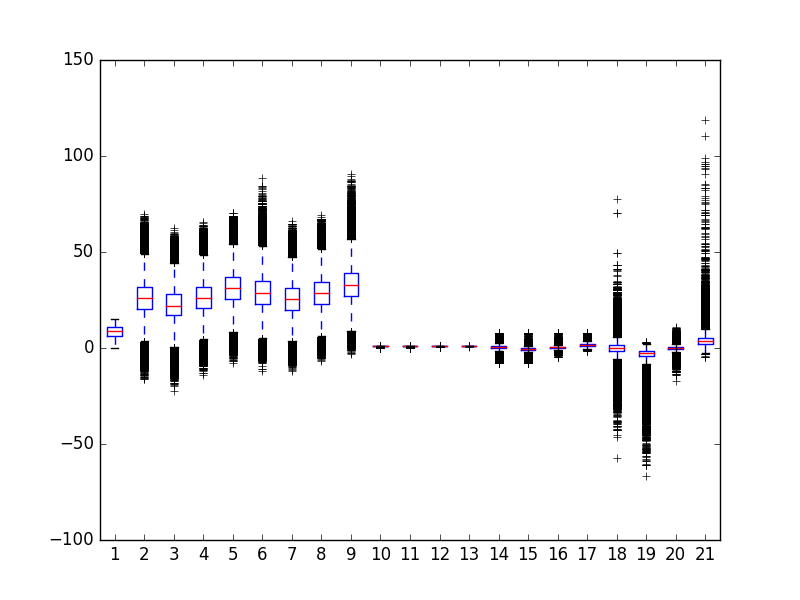
\includegraphics[width=0.5\textwidth]{fig/box_a_0.png}
	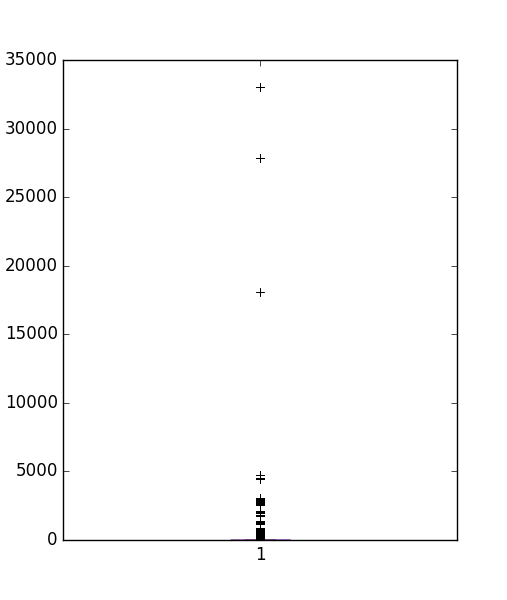
\includegraphics[width=0.4\textwidth]{fig/box_b_0.png}
	\caption{\small
		Left, box plot for columns of $A_0$,
        right, that for $b_0$.}
	\label{fig:box}
\end{figure}
